\section{QoI Scalability}
\label{sec:qoi_scalability}

Given the nonlinear returns of completeness and importance of timeliness outlined in the previous section, we contend that establishing limits of throughput is insufficient.  A non-QoI-aware approach ignores very useful information such as how changes in achievable data rates affect the actual utility of information at its destination as well as how changes in one QoI requirement can affect satisfiability of other requirements.  

For these reasons, we set the goal of determining the capacity of a network, and relatedly, the scalability achievable with respect to QoI requirements.  Previous methods that predict scalability do so by singling out a single bottleneck node and determining when it will be overloaded and drop packets. Here, we are forced to look at end to end flows and determine all contributors to delay, including MAC access, queuing delays, and multi-hop propagation to find the point at which timeliness requirements are violated or traffic load must be reduced thus adversely affecting completeness, leading to a more comprehensive analysis.

\subsection{QoI Satisfiability Framework}
In order to establish the framework, we examine an arbitrary flow, $F_1$, in the network that has a QoI requirement of $\mathbf{q} = \{C, T\}$, where $C$ is the minimum required completeness metric of choice, such as sum similarity as explained above, and $T$ is the required timeliness.  This flow will have a data size requirement, which is given by a chosen QoI function $Q(C)$.  Using the example application from \ref{sec:qoi_model}, for example, $Q(C)$ can return the number of images, $k_{req}$, required to achieve the requested completeness $C$. For simplicity, in this section, we use a fixed value for the data size requirement, but we expand our consideration to use a distribution for the data size requirement in our applications in Section \ref{sec:example_applications}.

Assuming each image has a size of $I_S$, then we can also use $B$ to describe the total number of bits required by the flow, $B=k_{req}*I_S$.  To match realistic network implications, we assume this data will be transmitted in a series of packets with size $P_S$ bits each. This packet size should include any bits necessary to implement techniques of error detection or correction that the network is utilizing. The number of packets per flow, then, is simply $P_N = \lceil B/P_S \rceil$.  We assume that each node in the network can transmit at $W$ bits per second when it is allocated media access.

Our goal is to establish the limits at which this arbitrary flow can no longer be completed with the QoI requirements satisfied.  {\color{blue}We build and explain our model for achieving this goal by working through an example TDMA line network, a portion of which is shown in Figures \ref{fig:delay_expl_fig_3} and \ref{fig:delay_expl_fig_4}. In this network, we assume a simple 3-slot TDMA scheme, which allows each node equal time access to the medium and, in this explanation, we remove any potential interference or hidden terminal issues. Recall that packet losses and retransmissions can be captured in this framework by using an \emph{effective} channel rate based on the physical channel rate and loss probability. Also, we discuss addressing non-TDMA networks, such as those that use a CSMA protocol, in Section \ref{sec:discussion}. }

The TDMA Slot assignments are labeled above each node in Figures \ref{fig:delay_expl_fig_3} and \ref{fig:delay_expl_fig_4}.  For simplicity, we will assume that one slot is appropriately sized to transmit a single packet, i.e., $T_{slot} = P_S/W$ and that packets use static routes calculated beforehand such that the overhead is not a consideration here.

{\color{blue}When calculating overall delay, four sources of delay are generally considered: processing, queuing, transmission, and propagation. We focus on transmission and queuing delay here and ignore processing and propagation delay, because the latter two are negligible compared to the former two for the wireless channel rates we are targeting in this work (on the order of MBs/sec or lower). If a higher level of precision is desired, however, propagation and processing delays can be added to the time to transmit each packet, which we adopt as the time duration of a time slot, $T_{slot}$ below, without changing the formulation of the framework. Furthermore, we do not incorporate consideration of excessive queuing delays since, as we stated in the model, our aim is to evaluate stable network traffic, which implies relatively small queue backlogs. %, and cases in which traffic is causing high queueing delays will not be providing timely delivery of data, and, thus is also out of the scope of this work.

%Similarly, delays associated with processing of packets may be added to this emission delay. We also ignore these delays here, though, and assume that packets can be just forwarded with a minimal amount of processing, e.g., only decoding the header to determine the next hop.

In developing our framework, we find it more intuitive to split the total delay into two functional parts, which we call $D_1$ and $D_2$. These two components do not separate queuing and transmission delays, but considering parts of each simultaneously. }
%We split the components of delay that contribute to the total delay of completing flow $F_1$ into two parts, $D_1$ and $D_2$. Each of these components capture part of the queuing delay and part of the transmission delay. 
The first contributor, $D_1$, is the end to end delay incurred by sending the $B$ bits across the designated path in the network. To quantify this delay, we must consider several factors beyond just the available bandwidth and number of packets in a flow. First, each node must share the channel with its one-hop neighbors, creating a factor of delay inversely proportional to the percentage of time access that it is allocated for a channel. We call this factor of delay the Channel Factor, which in this case is given by $CF = N_{frame}/N_{i}$, where $N_{i}$ is the number of slots allocated to node $i$ and $N_{frame}$ is the total number of slots in each frame. In this case, $N_{i} = 1, \forall i$ and $N_{frame} = 3$. 

The second factor to consider for $D_1$ is the fraction of allocated slots that are utilized by the node to serve flows other than $F_1$ that are either originating in or being routed through nodes on the path of flow $F_1$.  We call the total number of flows competing at node $i$ the Traffic Factor, $TF_i$, of that node.  For any flow, the maximum contributor to delay is the node along the path with the maximum $TF_i$, which we will just call $TF$ here.  More detail about determining this $TF$ is outlined in Appendix \ref{sec:derivation_TFs}.  Incorporating these considerations into a calculation for $D_1$, we achieve the following expression:  % NOTE: Maybe want to add a max-flow, min-cut argument here to help clarify?
\begin{equation}
	D_1 = T_{slot} \cdot P_N \cdot CF \cdot TF
\end{equation}

\begin{figure}
\begin{centering}
    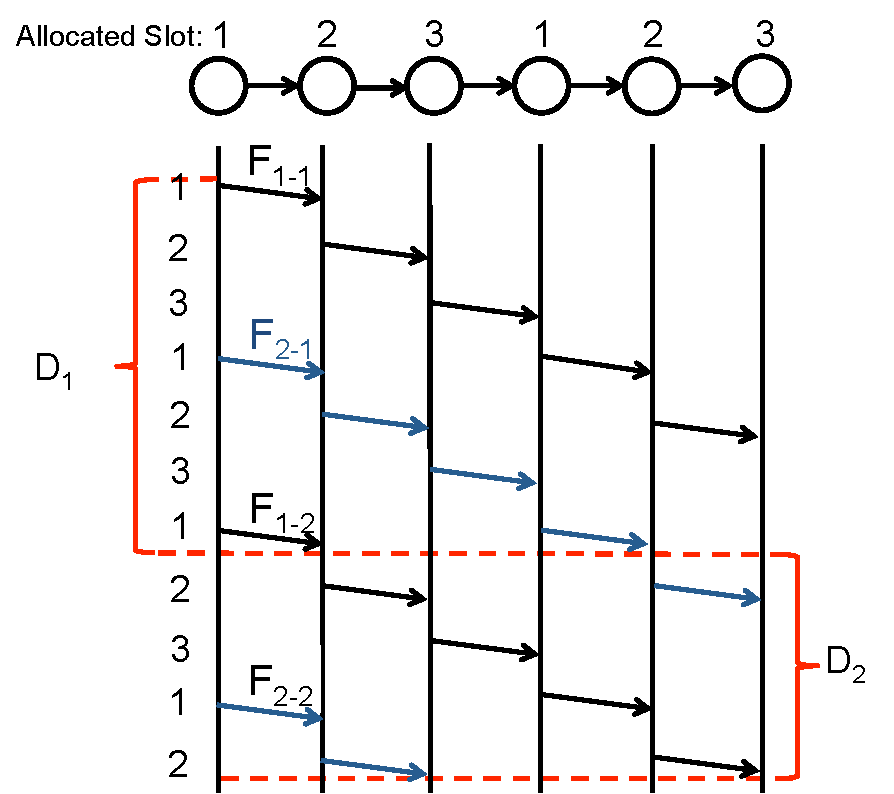
\includegraphics[scale=0.33]{figures/delay_limit_expl/fig_1_2.pdf}
    \caption{Example of line network using TDMA highlighting source of delays, $D_1$ and $D_2$.  (Node labels are slot assignments.)  Here, $TF = 2$, $CF = 3$, and $DF = 1$. }
    \label{fig:delay_expl_fig_3}
    \vspace{-6mm}
\end{centering}
\end{figure}

Figure \ref{fig:delay_expl_fig_3} depicts the delay of $D_1$ in a simple case of only two flows, $F_1$ and $F_2$, being present, in which case $TF = 2$.  In this example we use flows that consist of only $2$ ($F_{i-j}$ is packet $j$ in flow $i$) packets to portray the delay.  In most real applications, $P_N$ will be much larger, making $D_1$ a good approximation of this delay component.

\begin{figure}
\begin{centering}
    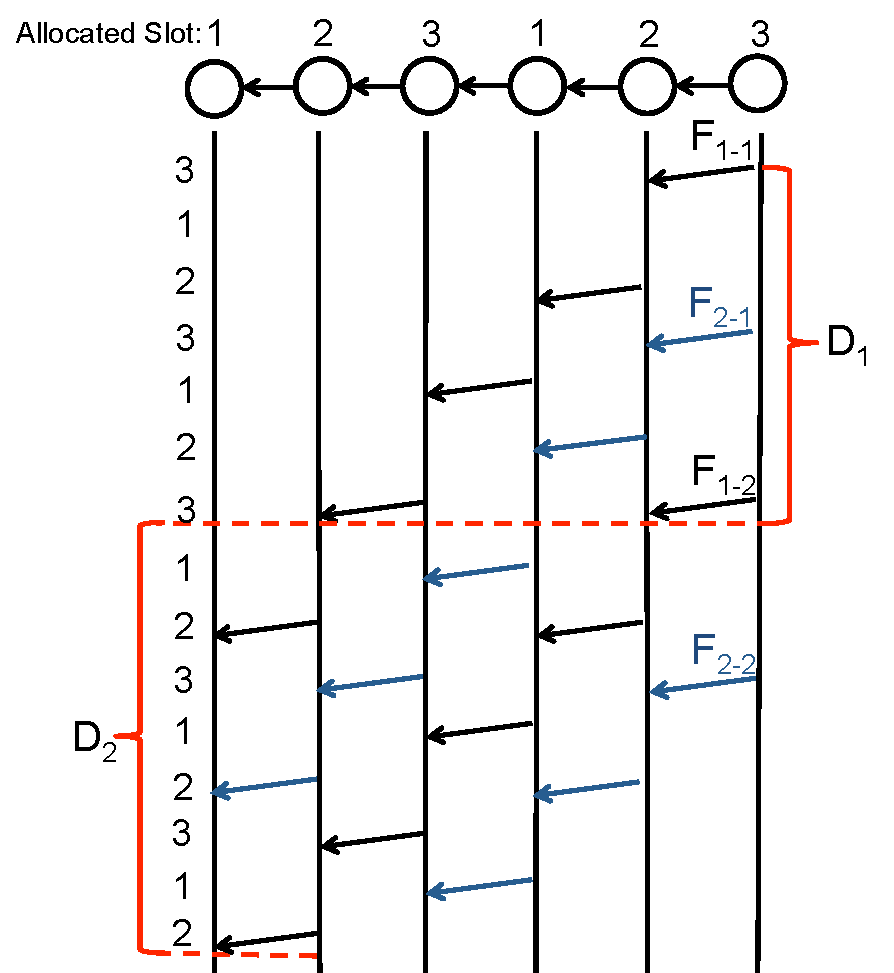
\includegraphics[scale=0.35]{figures/delay_limit_expl/fig_2_2.pdf}
    \caption{In the opposite direction, $DF = 2$. ($TF$ and $CF$ are unchanged here.)}
    \label{fig:delay_expl_fig_4}
    \vspace{-6mm}
\end{centering}
\end{figure}



\begin{table*}[]
\centering
\begin{tabular}{l|l|l|l|l|l|}
\cline{2-6}
%                            					 & \boldmath{$CF$}  			& \boldmath{$TF_{\mu}$}   			& \boldmath{$TF_{\sigma}$}										& \boldmath{$DF$}			& \boldmath{$PL_{max}$}	\\ \hline
                            					 & \boldmath{$CF$}  			& \boldmath{$\mu_{TF}$}   			& \boldmath{$\sigma_{TF}$}										& \boldmath{$DF$}			& \boldmath{$PL_{max}$}	\\ \hline
\multicolumn{1}{|l|}{\textbf{Clique}} & $N-1$ & $1$ & $0$ & $1$ & $1$ \\ \hline
\multicolumn{1}{|l|}{{\color{blue}\textbf{Star}}} & ${\color{blue}N-1}$ & ${\color{blue}N-2}$ & ${\color{blue}\sqrt{N-2}}$ & ${\color{blue}\frac{N}{2}}$ & ${\color{blue}2}$  \\ \hline
\multicolumn{1}{|l|}{\textbf{Line}} & $3$ & $\frac{N-1}{2}$ & $\sqrt{\frac{N-1}{2}}$ & $1.5$ & $N-1$ \\ \hline
\multicolumn{1}{|l|}{\textbf{Grid}} & $5$ & $\sqrt{N}$ &$N^{\frac{1}{4}}$ &  $2.5$ & $2 \cdot \sqrt{N}$ \\ \hline
\multicolumn{1}{|l|}{{\color{blue}\textbf{NSFNET}}}  & {\color{blue}$4$}  & {\color{blue}$2.15$}  & {\color{blue}$1.47$} &  {\color{blue}$2$}  & {\color{blue}$4$}  \\ \hline
\end{tabular}
\vspace{1mm}
\caption{CF, TF, DF, and PL values for example topologies}
\label{table:rf_ff_sf_values}
    \vspace{-4mm}
\end{table*}

\begin{table*}[]
\centering
\begin{tabular}{l|l|}
\cline{2-2}
                             & \multicolumn{1}{c|}{{\bf Equation}} \\ \hline
\multicolumn{1}{|l|}{\textbf{Clique}} & \multicolumn{1}{c|}{$W \cdot T - I_S \cdot k_{req} \cdot (N-1) \geq 0$}            \\ \hline
\multicolumn{1}{|l|}{{\color{blue}\textbf{Star}}}   & \multicolumn{1}{c|}{{\color{blue}$W \cdot T - (N-1) \cdot I_S \cdot k_{req} \cdot ( 1 + \frac{-\ln(\epsilon)}{2(N-1)(N-2)} \pm \sqrt{\frac{\ln(\epsilon)^2}{4(N-1)^2(N-2)^2} - 2\frac{\ln(\epsilon)}{(N-1)(N-2)}} )\cdot((N-1)(N-2)) - P_S \cdot N \geq 0$}}      \\ \hline
\multicolumn{1}{|l|}{\textbf{Line}}   & \multicolumn{1}{c|}{$W \cdot T - 3 \cdot I_S \cdot k_{req} \cdot (1 + \frac{-\ln(\epsilon)}{N-1} \pm \sqrt{\frac{\ln(\epsilon)^2}{(N-1)^2} - 4\frac{\ln(\epsilon)}{N-1}} ) \cdot \frac{N-1}{2} - P_S \cdot 1.5 \cdot (N-1) \geq 0$}       \\ \hline
\multicolumn{1}{|l|}{\textbf{Grid}}   & \multicolumn{1}{c|}{$W \cdot T - 5 \cdot I_S \cdot k_{req} \cdot (1 + \frac{-\ln(\epsilon)}{2\sqrt{N}} \pm \sqrt{\frac{\ln(\epsilon)^2}{4 \cdot N} - 2\frac{\ln(\epsilon)}{\sqrt{N}}} ) \cdot \sqrt{N} - P_S \cdot 2.5 \cdot (2 \cdot \sqrt{N} - 1) \geq 0$}      \\ \hline
\multicolumn{1}{|l|}{{\color{blue}\textbf{NSFNET}}}   & \multicolumn{1}{c|}{{\color{blue}$W \cdot T - 4 \cdot I_S \cdot k_{req} \cdot ( 1 + (\frac{-\ln(\epsilon)}{2 \cdot 2.15} \pm \sqrt{\frac{\ln(\epsilon)^2}{4 \cdot 2.15^2} - 2\frac{\ln(\epsilon)}{2.15}} ) \cdot 1.47) - P_S \cdot 2 \cdot 4 \geq 0$}}      \\ \hline
\end{tabular}
\vspace{1mm}
\caption{Scalability equations}
\label{table:scal_eqs}
    \vspace{-6mm}
\end{table*}

The second delay that exists is due to the packets travesing multi-hop paths. This delay is simply the time for a single packet to traverse the path length. Note that this delay is not necessarily just the path length multiplied by $T_{slot}$, because of possible channel contention and/or ordering constraints. We show here how ordering constraints impact this TDMA network. A node cannot forward a packet from the flow until it receives that packet from the previous hop. In our line network example, when the direction of the flow matches the nodes' schedule of slots $1-2-3-1-2-3$, as in Figure \ref{fig:delay_expl_fig_3}, each successive node receives a packet on the time slot before it is scheduled, resulting in no extra delay. For a flow in the opposite direction, though, where nodes are scheduled $3-2-1-3-2-1$, as in Figure \ref{fig:delay_expl_fig_4}, the first slot $1$ is not utilized, because the first node scheduled in time slot $1$ has not yet received a packet in the flow. Every other slot is wasted, on average, for the initialization of the flow, resulting in approximately twice the delay. We will use a term that we call the \emph{Delay Factor}, or $DF$, to account for this effect where it exists. The multi-hop queuing delay, then, is modeled by

\begin{equation}
	D_2 = T_{slot} \cdot DF \cdot (PL - 1)
\end{equation}
where $PL$ is the average path length.

We note several points about this delay factor.  First, in a loaded network, the nodes can and will serve other flows while awaiting the arrival of packets in this flow of focus. That utilized bandwidth does not, however, preclude this $DF$ impact on delay for the flow of interest, $F_1$.  Any node cannot serve $F_1$ until a packet from that flow has been received. Second, this delay is only accounted for once per flow because all other packets are pipelined. All other packets' delay is captured by the end to end delay, $D_1$.  This effect is best illustrated by examining the difference between $D_2$ in Figures \ref{fig:delay_expl_fig_3} and \ref{fig:delay_expl_fig_4}. Here, we see the multi-hop propagation requires twice the number of slots because every other slot is unused in $F_1$'s propagation.  In a TDMA model, the average delay factor is the average of all possible waiting times, which is equal to the number of slots in the schedule divided by $2$.
%To calculate a $DF$ for an entire network, we can calculate a $DF$ for each possible sample path and find the average of these values.  %For example, in the case of the line network with a $3$-slot schedule, $DF = 1$ in the direction for Figure \ref{fig:delay_expl_fig_3} and $DF = 2$ in the opposite direction shown in Figure \ref{fig:delay_expl_fig_4}, so the average $DF$ used to approximate average delay in the network is $DF_{line-avg}=1.5$.  

By adding the two components of delay, we can give a relation for a network that will successfully achieve an average flow's data and timeliness requirements:
\begin{equation*}
	T_{slot} \cdot P_N \cdot CF \cdot TF + T_{slot} \cdot DF \cdot (PL-1) \leq T
\end{equation*}
Recalling that the time of a slot is determined by %the size of a packet, $P_S$, and available channel rate, $W$, in the relation 
$T_{slot} = P_S/W$ %we can substitute to get
%\begin{equation*}
%	\frac{P_S}{W} \cdot P_N \cdot CF \cdot TF + \frac{P_S}{W} \cdot DF \cdot (PL-1) \leq T
%\end{equation*}
and that the total number of bits required for a flow $P_S \cdot P_N =  k_{req} \cdot I_S$ (where $k_{req}$ is given by a function of required QoI), we can get the following expression:
\begin{equation}
	W \cdot T - k_{req} \cdot I_S \cdot CF \cdot TF - P_S \cdot DF \cdot (PL-1) \geq 0	
	\label{eq:general_scal}
\end{equation}

Every network will have its own set of parameters that can be substituted into this general formula, providing a tool to approximate limitations and sensitivity to changes in specific parameters. To provide concrete examples of how the framework is used, next we give derived values of factors for a TDMA-based wireless network with a number of different topologies.




